\documentclass[35pt]{article}
\usepackage{ctex}
\usepackage{CJK}
\usepackage{picinpar,graphicx}
\usepackage{cite}
\usepackage{multirow}
\usepackage{hyperref,amsmath,amssymb,amscd}
\usepackage{setspace}
\setlength{\parindent}{2em}
\twocolumn
\begin{document}
\title{\textbf{Reverse Connection with Objectness Prior Networks for Object Detection I}}
\author{\textbf{Liangjie Cao}}
\date{\textbf{17 May 2018}}
\maketitle
\par
\setlength{\baselineskip}{15pt}
\section{Introduction}
\textbf{RON is a new framework like CNNs. CNNs\cite{name1} is a typical Special deep feedforward neural network. Driven by the success of these methods in Table~\ref{Table1}, a critical question arises: }is it possible to develop an elegant framework which can smartly associate the best of both methodologies and eliminate their major demerits? \textbf{Of course there is, That's why the authors build up RON. They propose RON object detection framework, which could associate the merits of region-based and region-free approaches.~\cite{name2}}
\par
\section{Related Work}
\textbf{Object detection is a fundamental and heavilyresearched task in computer vision area. It aims to localize and recognize every object instance with a bounding box.\cite{name3} The paper says the main advantage of these methods is high time-efficiency. For example, the feed-forward speed of YOLO is 45 FPS, 9× faster than Faster R-CNN.}
 \begin{table}[!htbp]
  \centering
 \begin{tabular}{|p{2cm}|p{2cm}|}
    \hline
    1 & region-free methods\\
    \hline
     2 & region-based methods\\
    \hline
  \end{tabular}
  \caption{\textbf{Two typical network methods}} \label{Table1}
  \end{table}
\par
\section{Network Architecture}
\textbf{RON object detection framework can be described in Figure~\ref{Figure1} Reverse connection enables former features to have more semantic information.  One reverse connection block is shown in Figure~\ref{Figure2}. Actually, there are four reverse fusion maps with different scales.  More importantly, as the reverse connection is learnable, the semantic information of former layers can be
significantly enriched. So this characteristic makes RON more effective in detecting all scales of objects compared with~\cite{name4}. I will continue learning in the following days.
}\\
 \begin{figure}[htbp]
 \centering
 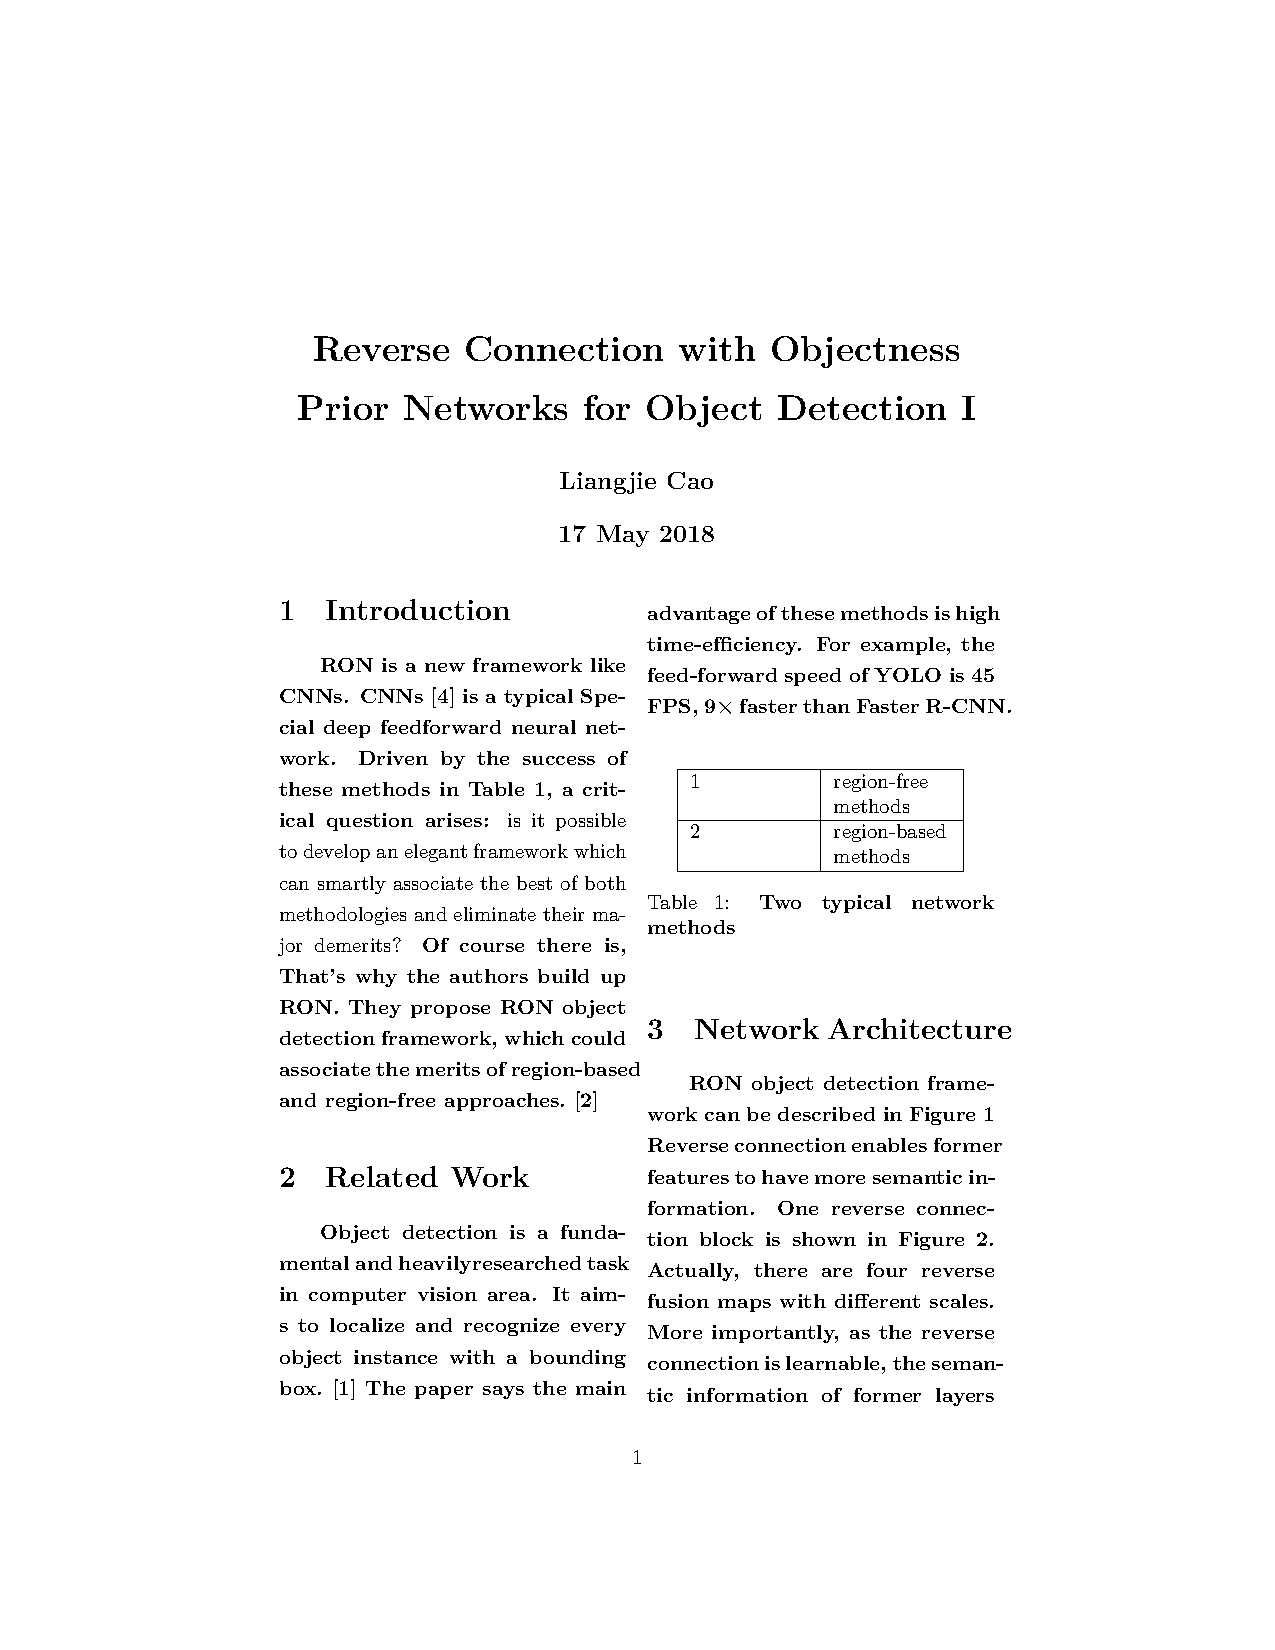
\includegraphics[width=0.5\textwidth]{RON.png}\\
 \caption{\textbf{RON object detection overview}}\label{Figure1}
  \centering
 \includegraphics[width=0.5\textwidth]{mod.png}\\
 \caption{\textbf{A reverse connection block}}\label{Figure2}
\end{figure}
  \bibliographystyle{plain}
\bibliography{yinyong1}
\end{document}

